\documentclass{beamer}
\usetheme[
  block=fill,
  background=dark,
  titleformat=smallcaps,
  progressbar=frametitle,
  numbering=none,
]{metropolis}

%----------------------------------------------------------------------------
% LoCo
%----------------------------------------------------------------------------
\setbeamertemplate{frametitle}[default][center]
\newcommand{\xx}{\pmb{\raisebox{-1.5pt}{$\mathcal{X}$}}}
\newcommand{\hh}{\pmb{h}}
\newcommand{\ii}{\pmb{i}}
\newcommand{\oo}{\pmb{o}}
\newcommand{\ff}{\pmb{f}}
\newcommand{\Ss}{\pmb{s}}
\newcommand{\bb}{\pmb{b}}

%Color
\definecolor{mDarkBrown}{HTML}{604c38}
\definecolor{mDarkTeal}{HTML}{23373b}
\definecolor{mLightBrown}{HTML}{EB811B}
\definecolor{mLightGreen}{HTML}{14B03D}
% Math
\usepackage{amsmath}
\usepackage{amssymb}
\usepackage{stmaryrd}
\usepackage{bm}
% Code listing
\usepackage{minted}
%\usemintedstyle{friendly}
\usemintedstyle{tango}
\usepackage{algorithm}
\usepackage[noend]{algpseudocode}

% Graphs
\usepackage{tikz}
\usetikzlibrary{calc, trees, fit, positioning}
\usepackage{pgfplots}
% Graphics
\usepackage{graphics}
\graphicspath{{figures/}} % Location of the graphics files

\newcommand\todo[1]{\textcolor{red}{#1}}
\newcommand{\w}[1]{\textit{"#1"}}
\newcommand{\sm}[1]{\text{\small{#1}}}

% Box macro
\newcommand{\ex}[2]{
  \vfill
  \begin{alertblock}{#1}
    #2
  \end{alertblock}
}
\newcommand\tsc[1]{\alert{\textsc{#1}}}

%----------------------------------------------------------------------------

% Beamer
\title{Differentiable Neural Computers}
\subtitle{Hybrid Computing using a neural network with dynamic external memory (Graves et al. 2016)}
\author{Konstantinos Kogkalidis}
\date{May 28, 2018}
\institute{Logic and Computation}

\begin{document}
	\maketitle
	
\begin{frame}{Overview}
	\alert{Differentiable Neural Computer}\\
	A recurrent neural network coupled with an external memory.
	
	\pause
	\begin{itemize}
	\item Extension of NTMs
	\begin{itemize}
		\pause
		\item End-to-end differentiable
		\pause
		\item Auto-associative memory
		\pause
		\item Turing complete
		\pause
		\item[+] Memory attention mechanisms
		\end{itemize}
	\pause
	\item Mimic mammalian biological memory
	\item Employ classical concepts of computation
	\end{itemize}
\end{frame}

\begin{frame}{Introduction: Motivation}
	\alert{Von Neumann architecture}
	\begin{figure}
	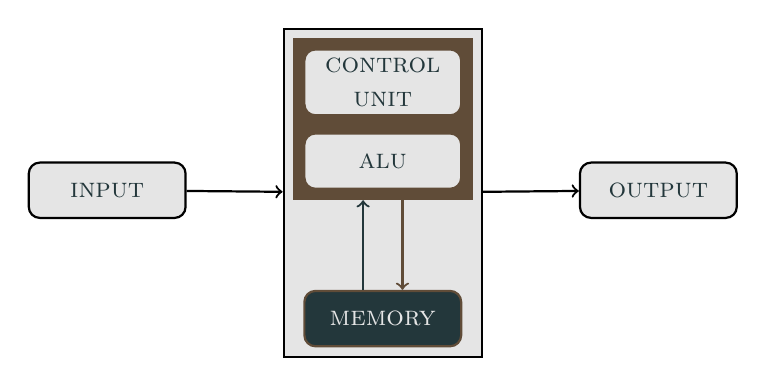
\begin{tikzpicture}
		[auto,
		block/.style ={rectangle, draw=mDarkBrown, thick, fill=gray!20, text width=5em, align=center, rounded corners, minimum height=2em},
		block2/.style ={rectangle, draw=mDarkBrown, thick, fill=mDarkTeal, text width=5em, align=center, rounded corners, minimum height=2em},
		block3/.style ={rectangle, draw=black, thick, fill=gray!20, text width=5em, align=center, rounded corners, minimum height=2em}]
		\draw (-1,0.63) node[block3] (i) {\textcolor{mDarkTeal}{\sc{input}}};
		\draw (6,0.63) node[block3] (o) {\textcolor{mDarkTeal}{\sc{output}}};
		
		\draw (2.5,-1) node[block2] (m) {\textcolor{gray!20}{\sc{memory}}};
		\draw (2.5,1) node[block] (a) {\textcolor{mDarkTeal}{\sc{alu}}};
		\draw (2.5,2) node[block] (c) {\textcolor{mDarkTeal}{\sc{control unit}}};
		
		\node[draw=mDarkBrown, thick, fill=mDarkBrown, fit=(a) (c)](Fit1) {};
		\draw (2.5,1) node[block] (a) {\textcolor{mDarkTeal}{\sc{alu}}};
		\draw (2.5,2) node[block] (c) {\textcolor{mDarkTeal}{\sc{control unit}}};
		
		\node[draw=black, thick, fill=gray!20, fit=(Fit1) (m)](Fit2) {};
		\node[draw=mDarkBrown, thick, fill=mDarkBrown, fit=(a) (c)](Fit1) {};
		\draw (2.5,1) node[block] (a) {\textcolor{mDarkTeal}{\sc{alu}}};
		\draw (2.5,2) node[block] (c) {\textcolor{mDarkTeal}{\sc{control unit}}};
		\draw (2.5,-1) node[block2] (m) {\textcolor{gray!20}{\sc{memory}}};

		\draw (i) edge [->, black, thick] (Fit2);
		\draw (Fit2) edge [->, black, thick] (o);
		\draw ($(m.north) + (0.25,0)$) edge [<-, mDarkBrown, thick] ($(Fit1.south) + (0.25, 0)$ );
		\draw ($(m.north) + (-0.25,0)$) edge [->, mDarkTeal, thick] ($(Fit1.south) + (-0.25, 0)$ );

	\end{tikzpicture}
	\end{figure}
\end{frame}



\begin{frame}{Introduction: Motivation}
	\begin{minipage}[t]{.44\textwidth}	
	\alert{Simple Neural Net}
	\begin{figure}[h!]
	\vspace{6.5pt}
	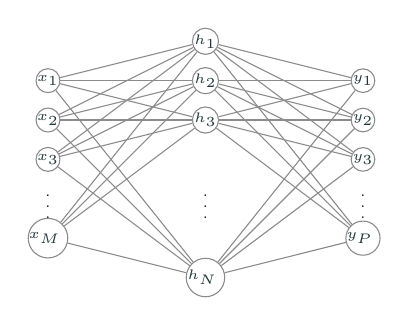
\begin{tikzpicture}[scale=.5]
		\foreach \y /\alph/\name in {
			0/x1/$x_1$,
		  	-1/x2/$x_2$,
		  	-2/x3/$x_3$,
		  	-4/xM/$x_M$
		 }{
		 	\node[circle, draw=gray!90, inner sep=0pt,minimum size=3mm,fill=white] (\alph) at (0,\y) {\tiny \textcolor{mDarkTeal}{\name}};
		 }
		 \node (x..) at (0,-3) {\tiny {\vdots}};
		 \foreach \y /\alph/\name in {
			1/h1/$h_1$,
		  	0/h2/$h_2$,
		  	-1/h3/$h_3$,
		  	-5/hN/$h_N$
		 }{
		 	\node[circle, draw=gray!90, inner sep=0pt,minimum size=3mm,fill=white] (\alph) at (4,\y) {\tiny \textcolor{mDarkTeal}{\name}};
		 }
		 \node (h..) at (4,-3) {\tiny {\vdots}};
		 \foreach \y /\alph/\name in {
			0/y1/$y_1$,
		  	-1/y2/$y_2$,
		  	-2/y3/$y_3$,
		  	-4/yP/$y_P$
		 }{
		 	\node[circle, draw=gray!90,inner sep=0pt,minimum size=3mm,fill=white] (\alph) at (8,\y) {\tiny \textcolor{mDarkTeal}{\name}};
		 }
		 \node (y..) at (8,-3) {\tiny {\vdots}};
		 \foreach \x in {x1, x2, x3, xM}
		 {\foreach \h in {h1, h2, h3, hN}
		 {\draw (\x) edge[gray!90] (\h);}}
		 \foreach \x in {h1, h2, h3, hN}
		 {\foreach \y in {y1, y2, y3, yP}
		 {\draw (\x) edge[gray!90] (\y);}}
	\end{tikzpicture}
	\end{figure}
	\vspace{10pt}
	\centering
	\small \alert{$y=g(h),\ h=f(x)$}\\
	No memory
	\end{minipage}
	\pause
	\hspace{1cm}
	\begin{minipage}[t]{.44\textwidth}	
	\alert{Recurrent Neural Net}
	\begin{figure}[h!]
	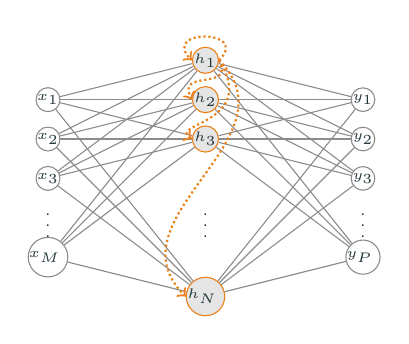
\begin{tikzpicture}[scale=.5]
		\foreach \y /\alph/\name in {
			0/x1/$x_1$,
		  	-1/x2/$x_2$,
		  	-2/x3/$x_3$,
		  	-4/xM/$x_M$
		 }{
		% 	\node[] (\alph) at (0,\y) {\name};
		 	\node[circle, draw=gray!90, inner sep=0pt,minimum size=3mm,fill=white] (\alph) at (0,\y) {\tiny \textcolor{mDarkTeal}{\name}};
		 }
		 \node (x..) at (0,-3) {\tiny {\vdots}};
		 \foreach \y /\alph/\name in {
			1/h1/$h_1$,
		  	0/h2/$h_2$,
		  	-1/h3/$h_3$,
		  	-5/hN/$h_N$
		 }{
		 	\node[circle, draw=mLightBrown, inner sep=0pt,minimum size=3mm,fill=gray!20] (\alph) at (4,\y) {\tiny \textcolor{mDarkTeal}{\name}};
		 }
		 \node (h..) at (4,-3) {\tiny {\vdots}};
		 \foreach \y /\alph/\name in {
			0/y1/$y_1$,
		  	-1/y2/$y_2$,
		  	-2/y3/$y_3$,
		  	-4/yP/$y_P$
		 }{
		 	\node[circle, draw=gray!90, inner sep=0pt,minimum size=3mm,fill=white] (\alph) at (8,\y) {\tiny \textcolor{mDarkTeal}{\name}};
		 }
		 \node (y..) at (8,-3) {\tiny {\vdots}};
		 \foreach \x in {x1, x2, x3, xM}
		 {\foreach \h in {h1, h2, h3, hN}
		 {\draw (\x) edge[gray!90] (\h);}}
		 \foreach \x in {h1, h2, h3, hN}
		 {\foreach \y in {y1, y2, y3, yP}
		 {\draw (\x) edge[gray!90] (\y);}}
		 \draw (h1.east) [->, densely dotted, thick, mLightBrown] .. controls +(0.8,0.8) and +(-0.8,0.8) .. (h1.west);
		 \draw (h1.east) [->, densely dotted, thick, mLightBrown] .. controls +(0.4,-0.8) and +(-0.4,0.8) .. (h2.west);
		 \draw (h1.east) [->, densely dotted, thick, mLightBrown] .. controls +(1,-1.6) and +(-0.6,0.4) .. (h3.west);
		 \draw (h1.east) [->, densely dotted, thick, mLightBrown] .. controls +(2,-2) and +(-2,2) .. (hN.west);
	\end{tikzpicture}
	\end{figure}
	\vspace{10pt}
	\centering
	\small{ \alert{$h(t)=f([x(t); h(t-1)])$}}\\
	Finite, non-contiguous memory
	\end{minipage}
\end{frame}

\begin{frame}{Approach}
	Train a RNN to act as a \alert{controller} to interact with a memory matrix of N (arbitrary many) addresses.
	\pause
	\begin{enumerate}
	\item \alert{Content Lookup}\\
		\begin{itemize}
		\item \alert{Attention} over memory defined by weightings $W \in \mathbb{R}^N$
		\item Compare controller output with memory objects (\alert{auto-associative memory})
		\item Allow partial matches  (\alert{pattern completion})
		\end{itemize}
	\pause
	\item \alert{Sequential Retrieval}
		\begin{itemize} 
		\item Fill $L \in \{0,1\}^{2N}$ indexing \alert{temporal transitions}
		\item \alert{Shift} operations defined by $LW,\ L^TW$
		\end{itemize}
	\pause
	\item \alert{Dynamic Allocation}
		\begin{itemize}
		\item Mark memory locations with $\{0,1\}$ to \alert{signal usage}
		\item Manipulate signals during R/W operations to enable \alert{reallocation}
		\item Generalization to \alert{unbounded memory}
		\end{itemize}
	\end{enumerate}
\end{frame}
	
\begin{frame}{Controller}
	A deep \alert{long short-term memory network} receiving 
	\[
	\xx_t=[ \pmb{x}_t; \pmb{r}_{t-1}^1; \dots ;\pmb{r}_{t-1}^R]
	\]
	and producing 
	\[
	(\pmb{v}_t,\pmb{\xi}_t)=\mathcal{N}([\xx_1;\dots;\xx_T];\theta)
	\]
	where $\mathcal{N}$ a set of state equations and $\theta$ their trainable parameters.
\end{frame}

\begin{frame}{Controller}
	A more detailed look into $\mathcal{N}$ and LSTMs:\\
	\begin{align}
	\ii_t^l &= \sigma(W_i^l[\xx_t;\hh_{t-1}^l;\hh_t^{l-1}]+\bb_i^l)   \tag{\alert{input gate}}\\
	\ff_t^l &= \sigma(W_f^l[\xx_t;\hh_{t-1}^l;\hh_t^{l-1}]+\bb_f^l)	\tag{\alert{forget gate}}\\
	\Ss_t^l &= \ff_t^l\Ss_{t-1}^l + \ii_t^ltanh(W_s^l[\xx_t;\hh_{t_1}^l;\hh_t^{l-1}] + \bb_s^l)		\tag{\alert{state}}\\
	\oo_t^l &= \sigma(W_o^l[\xx_t;\hh_{t-1}^l;\hh_t^{l-1}]+\bb_o^l)		\tag{\alert{output gate}}\\
	\hh_t^l &= \oo_t^ltanh(\Ss_t^l)		\tag{\alert{hidden}}\\
	\nonumber \\ 
	\pmb{v}_t &= W_y[\hh_t^1;\dots;\hh_t^L]		\tag{\alert{output vector}}\\
	\pmb{\xi}_t &= W_{\xi}[\hh_t^1;\dots;\hh_t^L]		\tag{\alert{interface vector}}
	\end{align}
\end{frame}

\begin{frame}{Controller}
	\alert{Single LSTM Layer}
	\begin{figure}
	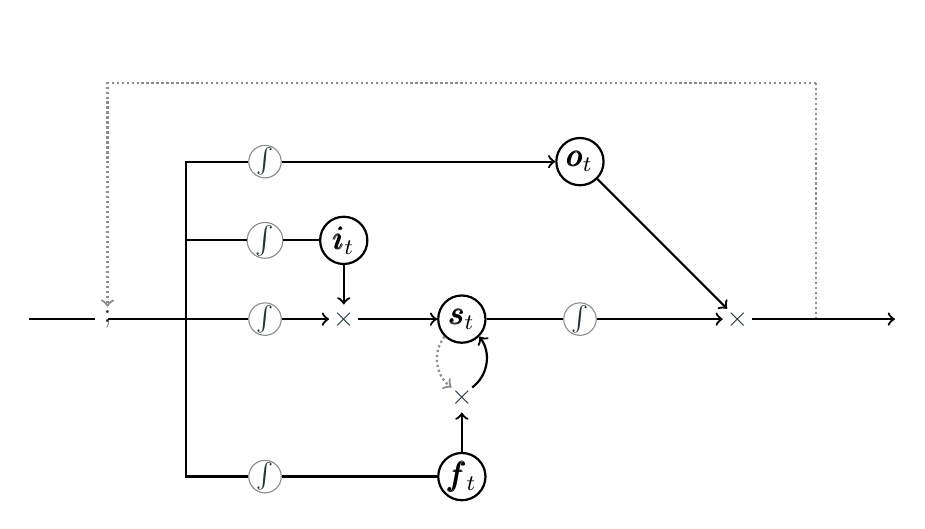
\begin{tikzpicture}[scale=0.5]
		%-------------------------------------------------------------------------------
		% LSTM
		%-------------------------------------------------------------------------------
		\node[circle, inner sep=0pt,minimum size=3mm,fill=white] (conc) 
			at (-0,6) {\textcolor{mDarkTeal}{$;$}};
		
		% outer box
		\draw[densely dotted, thick, gray!90] (18,6) -| (18,12);
		\draw[densely dotted, thick,->, gray!90] (18,12) -| (conc);
		%\draw[thick] (0,0) |- (18,12);
		%\draw[thick] (18,12) |- (0,0);
		
		% core nodes
		\node[circle, inner sep=0pt,minimum size=3mm,fill=white] (conc) 
			at (-0,6) {\textcolor{mDarkTeal}{$;$}};
		\node[circle, draw=black, thick, inner sep=0pt,minimum size=6mm,fill=white] (s) 
			at (9,6) {\large\textcolor{black}{$\Ss_t$}};
		\node[circle, inner sep=0pt,minimum size=3mm,fill=white] (fx) 
			at (9,4) {\textcolor{mDarkTeal}{$\times$}};
		\node[circle, draw=black, thick, inner sep=0pt,minimum size=6mm,fill=white] (f) 
			at (9,2) {\large\textcolor{black}{$\ff_t$}};
		\node[circle, draw=black, thick, inner sep=0pt,minimum size=6mm,fill=white] (i) 
			at (6,8) {\large\textcolor{black}{$\ii_t$}};
		\node[circle, inner sep=0pt,minimum size=3mm,fill=white] (ix) 
			at (6,6) {\textcolor{mDarkTeal}{$\times$}};
		\node[circle, draw=gray!90, inner sep=0pt,minimum size=3mm,fill=white] (id) 
			at (4,8) {\textcolor{mDarkTeal}{$\int$}};
		\node[circle, draw=gray!90, inner sep=0pt,minimum size=3mm,fill=white] (sd) 
			at  (4,6) {\small\textcolor{mDarkTeal}{$\int$}};
		\node[circle, draw=black, thick, inner sep=0pt,minimum size=6mm,fill=white] (o) 
			at (12,10) {\large\textcolor{black}{$\oo_t$}};
		\node[circle, inner sep=0pt,minimum size=3mm,fill=white] (ox) 
			at (16,6) {\textcolor{mDarkTeal}{$\times$}};
		\node[circle, draw=gray!90, inner sep=0pt,minimum size=3mm,fill=white] (od) 
			at (12,6) {\small\textcolor{mDarkTeal}{$\int$}};
		\node[circle, draw=gray!90, inner sep=0pt,minimum size=3mm,fill=white] (odd) 
			at (4,10) {\small\textcolor{mDarkTeal}{$\int$}};
		\node[circle, draw=gray!90, inner sep=0pt,minimum size=3mm,fill=white] (fd) 
			at (4,2) {\small\textcolor{mDarkTeal}{$\int$}};
		% recurrency
		\draw (f) edge[thick] (fd);
		\draw[thick] (fd) -| (2,6);
		\draw[thick] (2,6) |- (odd);
		\draw (odd) edge[->,thick] (o);
		\draw[thick] (2,6) |- (id);
		\draw (id) edge[thick] (i);
		% gates
		\draw (o) edge[->, thick] (ox);
		\draw (i) edge[->, thick] (ix);
		\draw (s) edge[->,bend right=45, thick, densely dotted, gray!90] (fx);
		\draw (s) edge[<-,bend left=45, thick] (fx);
		\draw (f) edge[->, thick] (fx);
		% forward
		\draw(-2,6) edge[thick] (conc);
		\draw (0,6) edge[thick] (sd);
		\draw (sd) edge[->, thick] (ix);
		\draw (ix) edge[->, thick] (s);
		\draw (s) edge[thick] (od);
		\draw (od) edge[->, thick] (ox);
		\draw (ox) edge[->, thick] (20,6);
		
		% labels
		\node[label=above:$\textcolor{white}{\xx_t}$] (x) at (-1,6) {};
		\node[label=above:$\textcolor{white}{\hh_t}$] (ht) at (19.5,6) {};
		\node[label=above:$\textcolor{white}{\hh_{t-1}}$] (x) at (9,12) {};
		\end{tikzpicture}
	\end{figure}
\end{frame}
\end{document}
